\documentclass[tikz,border=10pt]{standalone}
\usepackage{tikz}
\usetikzlibrary{positioning, calc, arrows.meta, fit}

\begin{document}
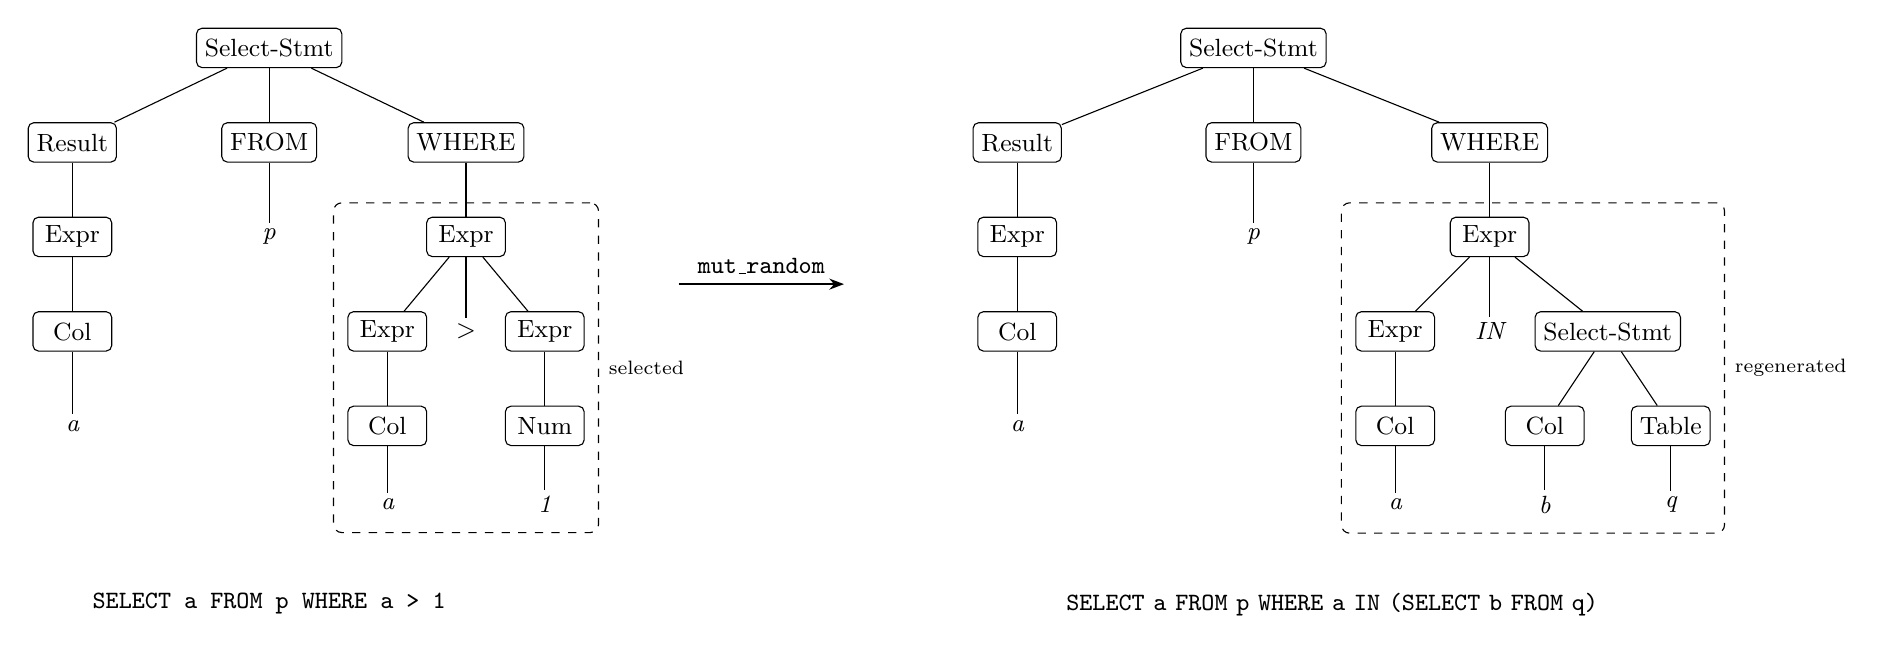
\begin{tikzpicture}[
    every node/.style={font=\small},
    % Non-terminal: small rounded rectangle, thin border
    nterm/.style={rectangle, rounded corners=2pt, draw=black, thin,
        minimum height=0.5cm, minimum width=1.0cm,
        inner sep=3pt, font=\small},
    % Terminal: italic, no border
    term/.style={font=\small\itshape, inner sep=2pt},
    % Edge style
    edge/.style={thin},
    % Dashed highlight box
    highlight/.style={draw=black, dashed, rounded corners=3pt,
        inner sep=5pt, thin},
    % Arrow between trees
    mutarrow/.style={-{Stealth[scale=0.8]}, thick},
]

% ====================================================
% LEFT TREE: SELECT a FROM p WHERE a > 1
% ====================================================
\begin{scope}[shift={(0,0)}]

    % Root
    \node[nterm] (L-root) at (0, 0) {Select-Stmt};

    % Level 1
    \node[nterm] (L-result) at (-2.5, -1.2) {Result};
    \node[nterm] (L-from) at (0, -1.2) {FROM};
    \node[nterm] (L-where) at (2.5, -1.2) {WHERE};

    % Level 2
    \node[nterm] (L-expr1) at (-2.5, -2.4) {Expr};
    \node[term] (L-p) at (0, -2.4) {p};
    \node[nterm] (L-expr2) at (2.5, -2.4) {Expr};

    % Level 3 (left branch)
    \node[nterm] (L-col1) at (-2.5, -3.6) {Col};

    % Level 3 (right branch: Expr > structure)
    \node[nterm] (L-expr3) at (1.5, -3.6) {Expr};
    \node[term] (L-gt) at (2.5, -3.6) {$>$};
    \node[nterm] (L-expr4) at (3.5, -3.6) {Expr};

    % Level 4
    \node[term] (L-a1) at (-2.5, -4.8) {a};
    \node[nterm] (L-col2) at (1.5, -4.8) {Col};
    \node[nterm] (L-num) at (3.5, -4.8) {Num};

    % Level 5
    \node[term] (L-a2) at (1.5, -5.8) {a};
    \node[term] (L-1) at (3.5, -5.8) {1};

    % Edges
    \draw[edge] (L-root) -- (L-result);
    \draw[edge] (L-root) -- (L-from);
    \draw[edge] (L-root) -- (L-where);
    \draw[edge] (L-result) -- (L-expr1);
    \draw[edge] (L-from) -- (L-p);
    \draw[edge] (L-where) -- (L-expr2);
    \draw[edge] (L-expr1) -- (L-col1);
    \draw[edge] (L-expr2) -- (L-expr3);
    \draw[edge] (L-expr2) -- (L-gt);
    \draw[edge] (L-expr2) -- (L-expr4);
    \draw[edge] (L-col1) -- (L-a1);
    \draw[edge] (L-expr3) -- (L-col2);
    \draw[edge] (L-expr4) -- (L-num);
    \draw[edge] (L-col2) -- (L-a2);
    \draw[edge] (L-num) -- (L-1);

    % Dashed rectangle around the replaced subtree (Expr under WHERE)
    \node[highlight, fit=(L-expr2)(L-expr3)(L-gt)(L-expr4)(L-col2)(L-num)(L-a2)(L-1),
        label={[font=\scriptsize, anchor=west]right:selected}] (L-box) {};

    % SQL label below
    \node[font=\small\ttfamily, anchor=north] at (0, -6.8)
        {SELECT a FROM p WHERE a > 1};

\end{scope}

% ====================================================
% ARROW BETWEEN TREES
% ====================================================
\draw[mutarrow] (5.2, -3.0) -- node[above, font=\small\ttfamily] {mut\_random} (7.3, -3.0);

% ====================================================
% RIGHT TREE: SELECT a FROM p WHERE a IN (SELECT b FROM q)
% ====================================================
\begin{scope}[shift={(12.5,0)}]

    % Root
    \node[nterm] (R-root) at (0, 0) {Select-Stmt};

    % Level 1
    \node[nterm] (R-result) at (-3.0, -1.2) {Result};
    \node[nterm] (R-from) at (0, -1.2) {FROM};
    \node[nterm] (R-where) at (3.0, -1.2) {WHERE};

    % Level 2
    \node[nterm] (R-expr1) at (-3.0, -2.4) {Expr};
    \node[term] (R-p) at (0, -2.4) {p};
    \node[nterm] (R-expr2) at (3.0, -2.4) {Expr};

    % Level 3 (left branch)
    \node[nterm] (R-col1) at (-3.0, -3.6) {Col};

    % Level 3 (right branch: Expr IN structure)
    \node[nterm] (R-expr3) at (1.8, -3.6) {Expr};
    \node[term] (R-in) at (3.0, -3.6) {IN};
    \node[nterm] (R-sel) at (4.5, -3.6) {Select-Stmt};

    % Level 4
    \node[term] (R-a1) at (-3.0, -4.8) {a};
    \node[nterm] (R-col2) at (1.8, -4.8) {Col};
    \node[nterm] (R-col3) at (3.7, -4.8) {Col};
    \node[nterm] (R-table) at (5.3, -4.8) {Table};

    % Level 5
    \node[term] (R-a2) at (1.8, -5.8) {a};
    \node[term] (R-b) at (3.7, -5.8) {b};
    \node[term] (R-q) at (5.3, -5.8) {q};

    % Edges
    \draw[edge] (R-root) -- (R-result);
    \draw[edge] (R-root) -- (R-from);
    \draw[edge] (R-root) -- (R-where);
    \draw[edge] (R-result) -- (R-expr1);
    \draw[edge] (R-from) -- (R-p);
    \draw[edge] (R-where) -- (R-expr2);
    \draw[edge] (R-expr1) -- (R-col1);
    \draw[edge] (R-expr2) -- (R-expr3);
    \draw[edge] (R-expr2) -- (R-in);
    \draw[edge] (R-expr2) -- (R-sel);
    \draw[edge] (R-col1) -- (R-a1);
    \draw[edge] (R-expr3) -- (R-col2);
    \draw[edge] (R-sel) -- (R-col3);
    \draw[edge] (R-sel) -- (R-table);
    \draw[edge] (R-col2) -- (R-a2);
    \draw[edge] (R-col3) -- (R-b);
    \draw[edge] (R-table) -- (R-q);

    % Dashed rectangle around the new subtree (Expr under WHERE)
    \node[highlight, fit=(R-expr2)(R-expr3)(R-in)(R-sel)(R-col2)(R-col3)(R-table)(R-a2)(R-b)(R-q),
        label={[font=\scriptsize, anchor=west]right:regenerated}] (R-box) {};

    % SQL label below
    \node[font=\small\ttfamily, anchor=north, text width=8cm, align=center] at (1.0, -6.8)
        {SELECT a FROM p WHERE a IN (SELECT b FROM q)};

\end{scope}

\end{tikzpicture}
\end{document}
